% mainfile: ../../../main.tex
\chapter{Dependence of \texorpdfstring{\acrshort{tmm}}{TMM} simulations on epoxy thickness}\label{ch:app:exp:tmm}
\begin{marginfigure}
    \centering
    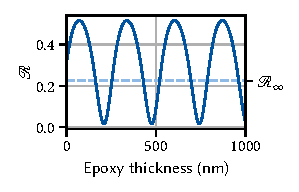
\includegraphics{img/pdf/experiment/reflectance_epoxy}
    \caption[\imgsource{img/py/experiment/tmm.py}]{
        Reflectance (top) and \gls{qw} absorptance (bottom) as function of epoxy thickness assuming coherent back-scattering.
        The period corresponds to the wavelength in epoxy, $\lambda_{\mr{epo}} = \lambda_0/n_{\mr{epo}}$.
    }
    \label{fig:app:exp:tmm:epoxy}
\end{marginfigure}

In \cref{sec:exp:tmm}, I carried out \gls{tmm} simulations of the membrane structure to elucidate the quenching of \gls{pl} intensity when focusing the laser on gates on the top or bottom side of the membrane.
There, I assumed incoherent scattering of photons at the epoxy/\ch{Si} interface below the membrane.
This assumption is based on the fact that \citet{Descamps2021} found the epoxy thickness, on the order of a few \unit{\micro\meter}, to vary significantly across the chip.
If the variation is fast enough, we can expect the phase of back-scattered photons to average out and hence destroy coherence.
Nonetheless, we should estimate the influence of coherent back-scattering.
\Cref{fig:app:exp:tmm:epoxy} shows the reflectance \reflectance and \gls{qw} absorptance \absorptance as function of the epoxy thickness.
The dashed line indicates the value resulting from the incoherent simulation.
Both quantities vary significantly with the epoxy thickness, but the incoherent values $\absorptance_\infty$ and $\reflectance_\infty$ are close to the average.
From the fact that neither the \gls{pl} nor the reflected laser intensity varies spatially by such large amounts in experiments, we can conclude that either the thickness variation is small enough to not play a significant role or that it varies fast enough to validate the assumption of incoherent back-scattering.

